\subsection{Secondary transfer to ds006780}

To test whether the head comparison transfers beyond the MIPDB cohort, we
evaluated a separate public EEG cohort from OpenNeuro ds006780. This extension
was motivated by the completed primary and capacity--data analyses, so it is a
secondary transfer experiment rather than a new blinded confirmatory test. The
external contract selected one predeclared resting-state recording per subject,
mapped the 64 BioSemi EEG channels to the canonical BioSemi-64 layout, and
preserved the acquisition reference because the source metadata did not specify
one. The frozen encoder and preprocessing remained unchanged.

The extension tested the final-layer mean-linear baseline and the
rich-statistics residual head at HBN training sizes $n=200$ and $n=800$, with
the ten fixed seeds 33--42. The sealed execution contained
\DsRunCount{} selected runs and
\DsPredictionCount{} subject-level prediction identities for
\DsSubjectCount{} eligible subjects. Table~\ref{tab:ds006780-summary}
shows the aggregate results and paired contrasts; Figure~\ref{fig:ds006780}
visualizes both absolute performance and the paired candidate--baseline
difference.

At $n=200$, the rich head was slightly below the matched baseline, with mean
paired difference \DsSecondaryDelta{} and interval
[\DsSecondaryCILow{},\,\DsSecondaryCIHigh{}]. At $n=800$, the
rich head was higher by \DsPrimaryDelta{} and all
\DsPrimaryWins{} observed seed-level differences were positive. However,
the subject-aware 95\% interval was
[\DsPrimaryCILow{},\,\DsPrimaryCIHigh{}], with width
\DsPrimaryCIWidth{} rather than the predeclared maximum width
\DsPrecisionMaxWidth{}. The precision gate therefore
\DsPrecisionGateStatus{}: the positive seed pattern is compatible with a
useful transfer gain, but the external cohort is not precise enough to
establish stable superiority. This result is complementary to, and does not
modify, the primary MIPDB decision.

\begin{table}[t]
  \centering
  \scriptsize
  \caption{Secondary ds006780 transfer. Pearson is the mean across ten seeds;
  seed SD is the across-seed standard deviation. The interval and paired
  difference are shown only for the rich head relative to the matched
  mean-linear baseline.}
  \label{tab:ds006780-summary}
  \input{../results/extensions/ds006780_external_v5/ds006780_summary.tex}
\end{table}

\begin{figure}[t]
  \centering
  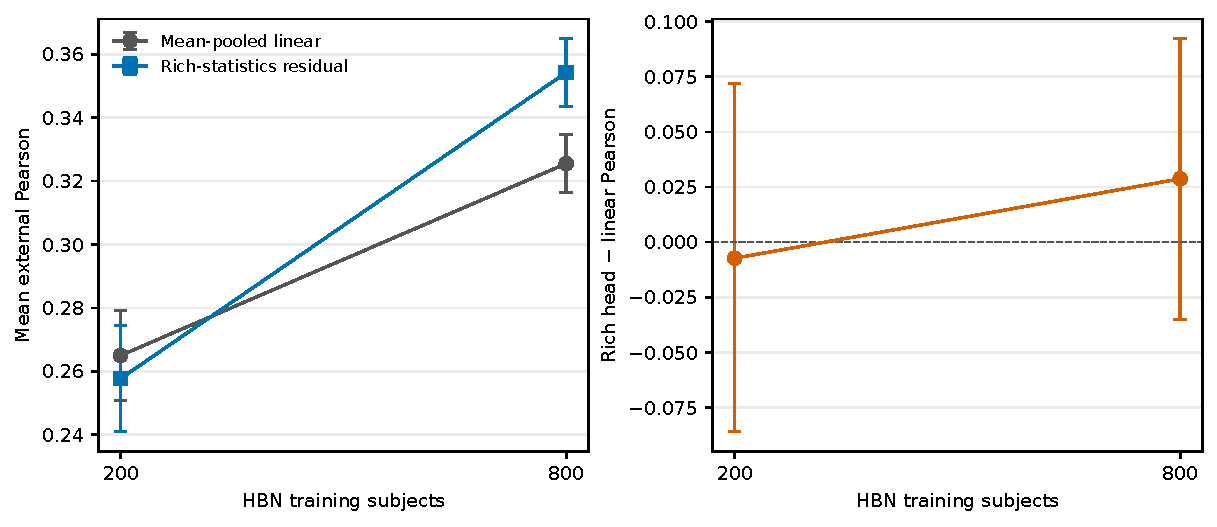
\includegraphics[width=0.98\linewidth]{../results/extensions/ds006780_external_v5/ds006780_external.pdf}
  \caption{Secondary ds006780 transfer. Left: absolute external Pearson scores
  with seed-level standard-deviation bars. Right: paired rich-head minus
  mean-linear Pearson differences with hierarchical seed--subject bootstrap
  intervals. Both intervals include zero.}
  \label{fig:ds006780}
\end{figure}
